\documentclass[journal]{IEEEtran}
% Preprint / draft formatting. Before IEEE Access submission, switch to the
% official ieeeaccess class from the IEEE Template Selector (see TEMPLATE_NOTES.md).
\usepackage{amsmath,amssymb,amsfonts}
\usepackage{booktabs}
\usepackage{graphicx}
\usepackage{url}
\usepackage{hyperref}
\usepackage{multirow}
\usepackage{xcolor}
\hyphenation{op-tical net-works semi-conduc-tor}

\begin{document}
\title{StructDay-Bench: A Protocol and Comparative Study for Structure-Conditioned Multi-Day Dietary Optimization from NHANES}

\author{Lei~Zhao%
\thanks{L.~Zhao and J.~Lu contributed equally.}%
\thanks{Corresponding authors: L.~Kang (kangling@neusoft.edu.cn), Q.~Guo (guoquan@neusoft.edu.cn).}%
, Jing~Lu, Yao~Wu, Xinning~Liu, Li~Han, Ling~Kang, Quan~Guo, and Fujin~Huang%
\thanks{L.~Zhao, J.~Lu, L.~Kang, and Q.~Guo are with Dalian Neusoft University of Information, Dalian, China.}%
\thanks{Y.~Wu, X.~Liu, and L.~Han are with the School of Software, Dalian Neusoft University of Information, Dalian, China.}%
\thanks{F.~Huang is with Dalian Scientific Test and Control Technology Institute, Dalian, China.}}

\markboth{IEEE Access (preprint draft)}%
{Zhao \MakeLowercase{\textit{et al.}}: StructDay-Bench}

\maketitle

\begin{abstract}
Personalized multi-day meal planning can be cast as constrained combinatorial optimization over fixed food portions: nutrient intervals must be met, meal occasions must remain plausible, and food identities should not repeat across successive days under a short wall-clock budget. Progress is hard to compare when each study redraws instances, alters budgets, or introduces a new solver together with a new problem definition. This paper contributes a \emph{benchmark and protocol}, not a new algorithm. We document how public NHANES individual-food recalls and linked FNDDS identifiers are transformed into optimization inputs---adult food-only cohorts, personalized nutrient intervals, demographic meal--category envelopes, and frozen candidate pools. We then freeze a confirmatory evaluation protocol (\texttt{external\_main\_v1}): twelve previously unexamined structure$\times$target units stratified by four prior difficulty labels, three seeds, 210\,s task and 30\,s per-day caps, seven-day horizon, and failure-retaining scoring. Ten existing search configurations---Aging-SMS, SMS-EMOA, AGE-MOEA/II, NSGA-II/III, R2HCA, scalar GA, generation- and wall-clock-aware RVEA adapters, and a CP-SAT band baseline---are compared on the same pools. Under the primary wall-clock-fair ledger, Aging-SMS delivers 212 days (148 all-band) across 36 tasks, while generation-fraction RVEA reaches 215/120 and a wall-clock APD RVEA adapter 204/113; CP-SAT-Band trails at 88/78. The resource is intended for preprint release and subsequent IEEE Access submission as a reproducible comparative study.
\end{abstract}

\begin{IEEEkeywords}
Dietary optimization, NHANES, benchmark, multi-objective evolutionary algorithms, evaluation protocol, meal structure, reproducibility.
\end{IEEEkeywords}

\section{Introduction}
\IEEEPARstart{D}{iet} composition is one of the earliest applied optimization problems~\cite{stigler1945}. Modern extensions incorporate acceptability, sustainability, and operational menu constraints~\cite{dooren2018,gazan2018,seljak2009,benvenuti2020}. When the decision variables are fixed-portion foods drawn from dietary surveillance, the task becomes a large binary selection problem with layered constraints: closed nutrient intervals, meal-slot legality, daily mass caps, and sequential exclusion of previously used food identities.

Population recalls from the National Health and Nutrition Examination Survey (NHANES), linked through the Food and Nutrient Database for Dietary Studies (FNDDS)~\cite{cdcDietary,usdaFndds}, supply empirical meal organization. Such data describe reported intake; they do not certify clinical optimality. Nonetheless, demographic meal$\times$category envelopes provide a transparent internal conformity criterion that can be shared across solvers.

IEEE Access regularly publishes dataset- and protocol-centric contributions that evaluate existing methods without proposing a new model~\cite{dales2021,cduie2023,nasbenchnlp2022,metaheuristics2021}. We follow that template for multi-day dietary optimization. Our contributions are:
\begin{enumerate}
\item a documented pipeline from NHANES raw transport files to frozen optimization instances;
\item a fixed confirmatory protocol with budgets, sampling rules, and outcome definitions;
\item a head-to-head comparison of established evolutionary and constraint baselines under that protocol.
\end{enumerate}
We deliberately exclude method papers that introduce new search operators from the claim of this manuscript; those belong in separate venues.

\paragraph{Relation to NutriOpt-Bench / RCFA.}
A separate experimental survey (NutriOpt-Bench) studies \emph{range-constrained food assembly} under equal evaluation budgets, with Feasible Hit Rate, Friedman ranks, and Kendall~$\tau$ across scale/sparsity/dimension axes. That work targets evolutionary-computation methodology on single-assembly interval boxes. StructDay-Bench is complementary and non-substitutable: it freezes multi-day sequential delivery under wall-clock caps, demographic meal$\times$category envelopes, food-identity nonrepetition across days, and delivery/all-band outcomes. We do not reuse RCFA FHR protocols, recipe-ceiling regimes, or cross-regime $\tau$ claims here.

\section{Related Work}
Mathematical programming reviews summarize nutrient-only and multi-criteria diet models~\cite{dooren2018,gazan2018}. Menu systems add operational constraints~\cite{seljak2009,benvenuti2020,sahin2024}. Evolutionary multi-objective algorithms---NSGA-II~\cite{deb2002}, NSGA-III~\cite{nsga3}, RVEA~\cite{rvea}, SMS-EMOA~\cite{sms2007}, AGE-MOEA variants~\cite{age1,age2}, and aging-based SMS adaptations~\cite{aging2025}---provide complementary selection pressures. Fair metaheuristic comparison itself is an active topic~\cite{metaheuristics2021}. Benchmark-style Access papers emphasize shared data, metrics, and baselines~\cite{dales2021,cduie2023,nasbenchnlp2022}. Our setting differs through fixed-portion binary genotypes, sequential food-ID bans, and wall-clock multi-day delivery rather than offline hypervolume on synthetic fronts or equal-evaluation FHR surveys of single-day interval assembly.

\section{From NHANES Raw Files to Optimization Inputs}
\label{sec:pipeline}
Fig.~\ref{fig:pipeline} summarizes the transformation. Upstream files are cycle-specific SAS transport tables (demographics, anthropometry, individual foods, supplements) plus FNDDS/FPED composition tables. We do not redistribute raw NHANES files; researchers must obtain them from NCHS under applicable terms~\cite{cdcDietary}.

\begin{figure*}[!t]
\centering
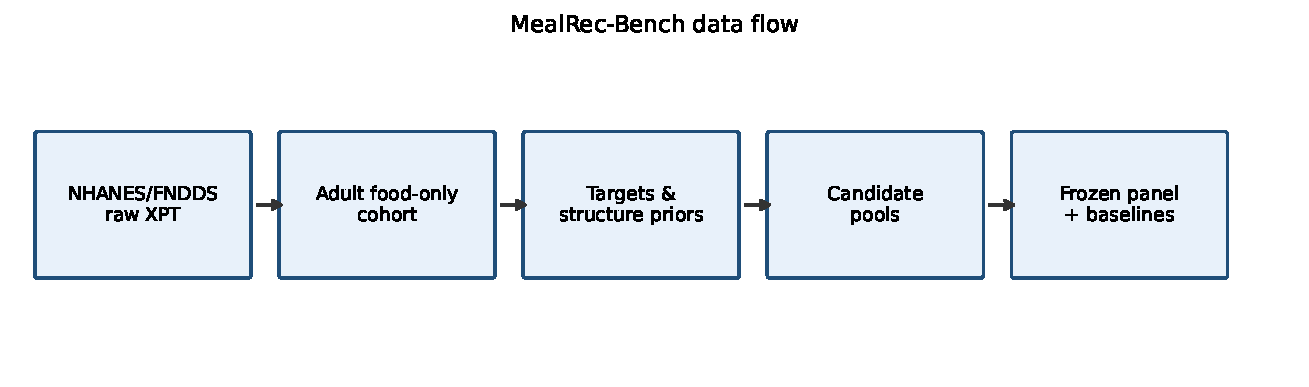
\includegraphics[width=0.95\textwidth]{figures/pipeline.pdf}
\caption{Data flow from NHANES/FNDDS raw tables to frozen confirmatory instances. Structure$\times$target units---not individual respondents---are the optimization work items.}
\label{fig:pipeline}
\end{figure*}

\subsection{Cohort construction}
Adult respondents ($\mathrm{RIDAGEYR}\ge 19$) are retained only if examination weight and height are present, at least one individual-food recall day exists, and dietary-supplement use is not indicated on the cycle-appropriate instrument (24-h totals or 30-day questionnaire). The design evaluates food-only nutrient gaps: supplements are excluded rather than treated as free micronutrient fillers.

For the reconciled release used here, standalone 2017--2018 is dropped in favour of the combined 2017--March 2020 release after an exact anthropometry/recall overlap audit. Processing counts (unweighted) include on the order of $10^5$ demographic records reduced to roughly $2.5\times 10^4$ retained respondent records and $>6\times 10^5$ individual-food rows; structure training uses a matched credible-day subset. These figures are processing volumes, not survey-weighted prevalence estimates.

\subsection{Health tags and nutrient intervals}
Examination, laboratory, and questionnaire fields yield binary condition tags and preference flags. Each participant maps to a dictionary of closed nutrient intervals $[L,U]$ (energy, macros, and conditional micronutrients). Many respondents share an identical target string; search is organized by the unique target together with a demographic structure key.

\subsection{Structure priors and pools}
Item-level recalls rebuild meal-share and day-mass summaries and meal$\times$FNDDS-major gram envelopes stratified by sex $\times$ BMI class $\times$ age band. Candidate pools apply plate-food exclusions, FPED coverage, meal-tag legality, single-item upper-bound filters, and cell locks when the learned upper envelope satisfies $h_i\le 0$. NHANES grams are preserved; FNDDS household measures are attached as display labels only. Each frozen instance stores the pool, envelopes, target, and mass cap $G_{\max}$.

\section{Problem and Protocol}
\label{sec:protocol}
\subsection{Decision variables and hard gates}
A day plan selects 5--15 pool rows. Hard gates (independent float64 validation) include nutrient intervals, cardinality, breakfast/lunch/dinner gram minima (30/50/50\,g), daily mass cap, condiment/oil/beverage dominance rules, meal-tag consistency, and forbidden-cell emptiness. Category gram envelopes remain soft for scoring; \emph{all-band} status means no upper-envelope violation on a delivered day. On this panel, effective non-forbidden lower bounds were zero, so all-band measures upper-envelope conformity rather than category coverage.

Across days within a task, accepted food identities (and configured FNDDS families) are removed from subsequent pools. Incomplete tasks remain in all denominators: we do not resample after observing solver success.

\subsection{Confirmatory panel}
Sampling seed 2026102612 excludes 150 previously exposed canonical identities (7831 eligible). Three units are drawn in each of four prior difficulty labels, yielding twelve structure$\times$target instances (Table~\ref{tab:panel}). Seeds $\{0,1,2\}$ produce 36 tasks per method. Budgets: 210\,s task wall clock, 30\,s per day, horizon seven days, population 200 for population-based adapters, shared top-eight observation mode.

\begin{table}[!t]
\caption{Confirmatory panel units (full IDs in \texttt{protocol/confirmatory\_panel\_selection.json}).}
\label{tab:panel}
\centering
\scriptsize
\begin{tabular}{@{}cll@{}}
\toprule
Difficulty & Instance ID & Structure key \\
\midrule
easy & \texttt{fbebc1d1bc5c13e8} & Male$|$normal$|$51--70 \\
easy & \texttt{fca20e2969a39437} & Male$|$obesity$|$31--50 \\
easy & \texttt{3c690b1c40609141} & Male$|$overweight$|$71+ \\
medium & \texttt{1fee2001494e90de} & Female$|$obesity$|$71+ \\
medium & \texttt{ed4b5ce589a8b282} & Male$|$obesity$|$51--70 \\
medium & \texttt{d3dfc39136a29917} & Male$|$overweight$|$71+ \\
hard & \texttt{8a3f005fa91b2e61} & Male$|$overweight$|$31--50 \\
hard & \texttt{084fdaa239107d4a} & Male$|$overweight$|$51--70 \\
hard & \texttt{e5c0f7decb17764f} & Male$|$overweight$|$71+ \\
extreme & \texttt{9aa236fbd9ee3a8c} & Female$|$normal$|$71+ \\
extreme & \texttt{cc75f7c978bdbf50} & Female$|$normal$|$31--50 \\
extreme & \texttt{7372adfc7e912a61} & Female$|$obesity$|$71+ \\
\bottomrule
\end{tabular}
\end{table}

\subsection{Baselines (existing algorithms only)}
All methods share pools, repairs, validation, and deadlines. Compared adapters: Aging-SMS (finite age-init correction), SMS-EMOA, AGE-MOEA, AGE-MOEA-II, NSGA-II, NSGA-III, R2HCA, scalar GA, RVEA with generation-fraction angle-penalized distance (APD), RVEA with wall-clock-fraction APD, and CP-SAT-Band (constraint program over category bands without evolutionary search). We report both RVEA adapters because generation-fraction APD can overstate progress under wall-clock accounting~\cite{metaheuristics2021}.

\section{Results}
\label{sec:results}
Table~\ref{tab:totals} aggregates delivered and all-band days over 36 tasks. Under wall-clock-fair reading, Aging-SMS (212/148) dominates wall-clock RVEA (204/113) and the remaining evolutionary adapters on the joint (days, all-band) profile, while generation-fraction RVEA posts the highest raw day count (215) with weaker envelope conformity (120). CP-SAT-Band returns substantially fewer days (88/78), indicating that band-focused exact search alone is insufficient under the sequential multi-day budget. Program errors were zero for listed methods on this panel.

\begin{table}[!t]
\caption{Aggregate outcomes on the confirmatory panel (36 tasks each). Higher is better. BELEX and other new operators are excluded from this benchmark ledger.}
\label{tab:totals}
\centering
\begin{tabular}{@{}lrrr@{}}
\toprule
Method & Days & All-band & Notes \\
\midrule
RVEA (gen.-frac.\ APD) & 215 & 120 & time-accounting caveat \\
Aging-SMS & 212 & 148 & primary wall-clock baseline \\
GA & 211 & 143 & scalar \\
NSGA-III & 210 & 141 & \\
NSGA-II & 208 & 141 & \\
R2HCA & 208 & 138 & \\
AGE-MOEA-II & 205 & 141 & \\
SMS-EMOA & 205 & 133 & \\
AGE-MOEA & 204 & 141 & \\
RVEA (wall-clock APD) & 204 & 113 & fair APD schedule \\
CP-SAT-Band & 88 & 78 & non-evolutionary \\
\bottomrule
\end{tabular}
\end{table}

Difficulty-stratified patterns (Aging-SMS) show near-ceiling easy/hard day delivery with larger all-band gaps on medium units, motivating stratified reporting rather than a single mean rank. Full per-task matrices and instance identifiers are released under \texttt{protocol/} and \texttt{results/}.

\section{Discussion}
A shared protocol changes the interpretation of ``better.'' Day count alone favours generation-fraction RVEA; envelope conformity and wall-clock APD reverse that conclusion relative to Aging-SMS. Benchmark users should therefore publish both delivered and all-band totals, declare APD schedules, and retain failures. Limitations include: no human palatability ratings; no external diet-quality index as a hard gate; structure$\times$target sampling rather than respondent-level hold-out; and adapters that are batch implementations of literature methods, not byte-identical reference codes. Clinical suitability is not claimed~\cite{cdcEthics}.

\section{Conclusion}
StructDay-Bench documents an NHANES-to-instance pipeline, freezes a confirmatory multi-day protocol, and compares existing algorithms under identical pools and budgets. Aging-SMS is a strong wall-clock baseline on the released panel; fair RVEA accounting matters. We release the manuscript, protocol JSON, and aggregate tables for preprint posting, with IEEE Access submission planned after official template packaging and public code linkage.

\section*{Data and Code Availability}
NHANES/FNDDS raw files must be obtained from NCHS/USDA. Protocol JSON, panel selection, and aggregate CSVs accompany this repository. Runtime extraction for public release is staged separately. Generated aggregates: CC~BY~4.0.

\section*{Acknowledgments}
The authors thank NHANES participants and NCHS staff. Assistive tools (ChatGPT/Codex, Cursor) supported drafting and engineering; human authors remain responsible for analyses and text.

\begin{thebibliography}{00}
\bibitem{stigler1945} G.~J. Stigler, ``The cost of subsistence,'' \emph{J. Farm Econ.}, vol.~27, no.~2, pp.~303--314, 1945.
\bibitem{dooren2018} C.~van Dooren, ``A review of the use of linear programming to optimize diets\ldots,'' \emph{Front. Nutr.}, vol.~5, p.~48, 2018.
\bibitem{gazan2018} R.~Gazan \emph{et al.}, ``Mathematical optimization to explore tomorrow's sustainable diets,'' \emph{Adv. Nutr.}, vol.~9, no.~5, pp.~602--616, 2018.
\bibitem{seljak2009} B.~K. Seljak, ``Computer-based dietary menu planning,'' \emph{J. Food Compos. Anal.}, vol.~22, pp.~698--704, 2009.
\bibitem{benvenuti2020} L.~Benvenuti and A.~De Santis, ``Making a sustainable diet acceptable,'' \emph{Front. Nutr.}, 2020.
\bibitem{cdcDietary} CDC/NCHS, ``NHANES dietary data.'' [Online]. Available: \url{https://wwwn.cdc.gov/nchs/nhanes/}
\bibitem{usdaFndds} USDA ARS, ``Food and Nutrient Database for Dietary Studies.'' [Online].
\bibitem{cdcEthics} CDC/NCHS, ``NCHS Ethics Review Board.'' [Online].
\bibitem{deb2002} K.~Deb \emph{et al.}, ``A fast and elitist multiobjective genetic algorithm: NSGA-II,'' \emph{IEEE Trans. Evol. Comput.}, vol.~6, no.~2, pp.~182--197, 2002.
\bibitem{nsga3} K.~Deb and H.~Jain, ``NSGA-III,'' \emph{IEEE Trans. Evol. Comput.}, vol.~18, no.~4, pp.~577--601, 2014.
\bibitem{rvea} R.~Cheng \emph{et al.}, ``RVEA,'' \emph{IEEE Trans. Evol. Comput.}, vol.~20, no.~5, pp.~773--791, 2016.
\bibitem{sms2007} N.~Beume \emph{et al.}, ``SMS-EMOA,'' \emph{Eur. J. Oper. Res.}, vol.~181, no.~3, pp.~1653--1669, 2007.
\bibitem{age1} A.~Panichella, ``AGE-MOEA,'' in \emph{GECCO}, 2019.
\bibitem{age2} A.~Panichella, ``AGE-MOEA-II,'' in \emph{GECCO}, 2022.
\bibitem{aging2025} Y.~Li, W.~Zheng, and B.~Doerr, ``Aging mechanisms for evolutionary multiobjective optimization,'' \emph{IEEE Trans. Evol. Comput.}, 2025.
\bibitem{metaheuristics2021} A.~Kazikova \emph{et al.}, ``How does the number of objective function evaluations impact\ldots,'' \emph{IEEE Access}, vol.~9, pp.~44032--44048, 2021.
\bibitem{dales2021} N.~M. Singer and V.~K. Asari, ``DALES Objects,'' \emph{IEEE Access}, 2021, doi: 10.1109/ACCESS.2021.3094127.
\bibitem{cduie2023} A.~Saleem \emph{et al.}, ``CDUIE underwater enhancement evaluation,'' \emph{IEEE Access}, 2023, doi: 10.1109/ACCESS.2023.3240648.
\bibitem{nasbenchnlp2022} N.~Klyuchnikov \emph{et al.}, ``NAS-Bench-NLP,'' \emph{IEEE Access}, vol.~10, pp.~45736--45747, 2022.
\bibitem{sahin2024} Open-source multi-objective menu planning software, \emph{SoftwareX}, 2024.
\end{thebibliography}

\begin{IEEEbiography}{Lei Zhao}
is with Dalian Neusoft University of Information. Research interests include evolutionary optimization and computational nutrition.
\end{IEEEbiography}
\begin{IEEEbiography}{Jing Lu}
is with Dalian Neusoft University of Information.
\end{IEEEbiography}
\begin{IEEEbiography}{Yao Wu}
is with the School of Software, Dalian Neusoft University of Information.
\end{IEEEbiography}
\begin{IEEEbiography}{Xinning Liu}
is with the School of Software, Dalian Neusoft University of Information.
\end{IEEEbiography}
\begin{IEEEbiography}{Li Han}
is with the School of Software, Dalian Neusoft University of Information.
\end{IEEEbiography}
\begin{IEEEbiography}{Ling Kang}
is with Dalian Neusoft University of Information.
\end{IEEEbiography}
\begin{IEEEbiography}{Quan Guo}
is with Dalian Neusoft University of Information.
\end{IEEEbiography}
\begin{IEEEbiography}{Fujin Huang}
is with Dalian Scientific Test and Control Technology Institute.
\end{IEEEbiography}

\end{document}
